The SM~\cite{Salam:1968rm, Glashow:1961tr, Weinberg:1967tq, Herrero:1998eq, Cottingham:2007zz} has been a stupendous success in predicting and explaining the physics phenomena of the elementary particles.
However, the SM leaves several open questions unanswered as mentioned in Sect.~\ref{sec:sm_bsm}.
Many different models of new physics were proposed to explain those unanswered questions.
Among these new models, \textit{supersymmetry} (SUSY)~\cite{Wess:1974tw, Lykken:1996xt, Drees:1996ca, Martin:1997ns, Bilal:2001nv, Argyres:2001eva, Peskin:2008nw, Aitchison:2005cf, Shadmi:2017qdk} is favored by most physicists.
The SUSY proposed by Wess and Zumino~\cite{Wess:1974tw} in the early 1970s is a symmetry that relates bosonic and fermionic degrees of freedom.
It extends the SM by requiring that every SM boson/fermion has a fermonic/bosonic supersymmetric partner and vice versa.
The reason why physicists favor SUSY is described in Sect.~\ref{sec:susy_why_susy} and the introduction of the SUSY as well as the formalism are given in Sect.~\ref{sec:susy_intro}.
The \textit{Radiative Natural SUSY} (RNS) and the \textit{Non-Universal Higgs Mass model} with two extra parameters (NUHM2) are described in Sect.~\ref{sec:susy_rns} and ~\ref{sec:susy_nuhm2}, respectively.

%%%
%%%
%%%

\section{Why supersymmetry}
\label{sec:susy_why_susy}
The SM leaves several unanswered questions; for example, the hierarchy problem (Sect.~\ref{subsec:sm_hierarchy_problem}), what are the candidates of dark matter (Sect.~\ref{subsec:sm_dm}), and why don't the running coupling constants unify at GUT level (Sect.~\ref{subsec:sm_grand_unification}).
SUSY provides good explanations for these questions.

%%%
%%%
%%%

%\begin{figure}[htbp]
%\begin{center}
%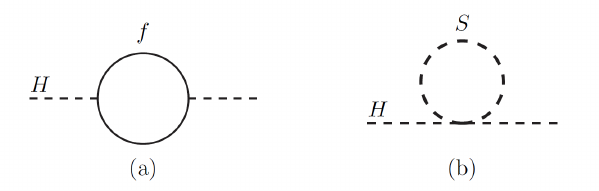
\includegraphics[scale=0.5]{Figure-1-One-loop-quantum-corrections-to-the-Higgs-squared-mass-parameter-m-2-H-from.png}
%\caption{The Feynman diagram for the one loop correction to the Higgs squared mass due to (a) a fermion $f$ and (b) a scalar $S$.
%The figure is taken from~\cite{Martin:1997ns}.}
%\label{fig:susy_one_loop_corrections}
%\end{center}
%\end{figure}
\begin{figure}[htbp]
    \begin{center}
        \begin{subfigure}[b]{0.48\textwidth}
            \begin{center}
                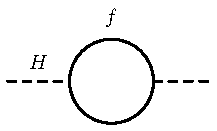
\includegraphics[scale=1]{one-loop-correction-1.pdf}
                \caption{}
            \end{center}
        \end{subfigure}%
        \begin{subfigure}[b]{0.48\textwidth}
            \begin{center}
                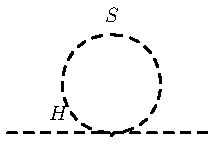
\includegraphics[scale=1]{one-loop-correction-2.pdf}
                \caption{}
            \end{center}
        \end{subfigure}
    \end{center}
    \caption{The Feynman diagram for the one loop correction to the Higgs squared mass due to (a) a fermion $f$ and (b) a scalar $S$~\cite{Martin:1997ns}.}
    \label{fig:susy_one_loop_corrections}
\end{figure}

\subsubsection{The hierarchy problem}
\label{subsubsec:susy_hierarchy_problem}
The SM predicts the Higgs squared mass diverges at the Plank scale $\sim 10^{19}$~{\GeV}.
However, the fact that $W^{\pm}$ and $Z^{0}$ gauge bosons obtain their finite mass through the Higgs mechanism indicates the Higgs squared mass must be finite.
Figure~\ref{fig:susy_one_loop_corrections} shows the Feynman diagram for the one loop correction to the Higgs squared mass due to a fermion $f$ and a scalar $S$.
The corrections are
%
\begin{align}
    \Delta m_{H}^{2} &= - \frac{|\lambda_{f}^{2}|}{8\pi^{2}} \Lambda_{UV}^{2} + \cdots, \quad \mathrm{fermion}\\
    \Delta m_{H}^{2} &= \frac{\lambda_{S}}{16\pi^{2}} \Lambda_{UV}^{2} + \cdots, \quad \mathrm{boson}
\end{align}
%
where the $\Lambda_{UV}$ is an ultraviolet momentum cutoff which is valid up to the Plank scale $10^{19}$~{\GeV}.
The corrections diverge when $\Lambda_{UV}$ becoming very large.
Because the contributions from the fermion and scalar loops have opposite sign, the divergence contributions can be canceled out if there is a scalar loop for each fermonic loop.
The SUSY predicts the existence of the bosonic/fermonic sparticles, therefore, if $\lambda_{S} = 2 |\lambda_{f}^{2}|$ then the SUSY maintain the finiteness of the Higgs squared mass in a natural way.

%%%
%%%
%%%

\subsubsection{Dark matter}
\label{subsubsec:susy_dark_matter}
Dark matter (DM) makes up about 27\% of the universe and might originate from neutral relics from the early universe.
The cosmologic observations of DM indicate that the dark matter should be electrically neutral, cold, massive, and participates only in weak and gravitational interactions.
Therefore, the DM candidate should be a new particle that is a \textit{weakly interacting massive particle} (WIMP).
SUSY requires that all the sparticles are produced in pairs that decay into stable \textit{lightest SUSY particles} (LSP) with odd number.
If there are a lot of sparticles produced in the early Universe, they will have to decayed to LSPs and remain until the present day because the LSP is stable.
The LSP is a weakly interacting massive particle.
LSPs do not interact electromagnetically so they cannot be scattered by photons and thus are dark.
There are three kinds of LSP that could be a possible DM candidate: the lightest \textit{neutralino}, the lightest \textit{sneutrino} and the \textit{gravitino}.

%%%
%%%
%%%

\subsubsection{Grand Unification}
\label{subsubsec:susy_gut}
Grand Unified Theories (GUT) try to unify the strong and electroweak interactions.
There will be only one interaction and one coupling constant at the GUT scale ($\approx 10^{16}$~{\GeV}).
However, the current coupling constants for electromagnetic, weak, and strong interactions do not unify at the GUT scale as shown in the left hand side of Fig.~\ref{fig:sm_coulping_constants}.
This problem can be solved by introducing the SUSY which modifies the renormalization group equations and makes the running gauge couplings converge at the GUT scale.
The right hand side of Fig.~\ref{fig:sm_coulping_constants} shows the running gauge couplings in SUSY.

%%%
%%%
%%%

\section{Introduction to supersymmetry}
\label{sec:susy_intro}
An brief overview of the SUSY are introduced in this section.
Firstly, the mathematical foundation of the SUSY, superalgebra, is described in Sect.~\ref{subsec:susy_superalgebra} followed by the superspace and superfields in Sect.~\ref{subsec:susy_superspace_and_superfields}.

%%%
%%%
%%%

\subsection{Superalgebra}
\label{subsec:susy_superalgebra}

%%%
%%%
%%%

\subsubsection{Poincar\'{e} algebra}
\label{subsubsec:susy_poincare}
The SUSY is based on superalgebra which is an extension of space-time Poincar\'{e} algebra.
The Poincar\'{e} group is a product of the Lorentz group and the group of translations in space-time.
A Lorentz group must satisfies the commutation relations
%
\begin{equation}
    [J^{+}_{i}, J^{+}_{j}] = i \epsilon_{ijk} J^{+}_{k}, \quad 
    [J^{-}_{i}, J^{-}_{j}] = i \epsilon_{ijk} J^{-}_{k}, \quad 
    [J^{+}_{i}, J^{-}_{j}] = 0 \quad ,
    \label{eq:susy_Lorentz_commutation_relations}
\end{equation}
%
where $i, j, k = 1, 2, 3$.
If the six Lorentz group generators are combined into an antisymmetric second rank tensor generator $M_{\mu\nu}$ where $M_{ij} = \epsilon_{ijk}J_{k}$ and $M_{0i} = -M_{i0} = -K_{i}$\footnote{The $J_{i}$ and $K_{i}$ with $i=1,2,3$ are rotation and boost generators in 3-dimensions, respectively. And the ladder operators are defined as $J_{i}^{\pm} = \frac{1}{2} (J_{i} \pm i K_{i})$.} and the generator of the translation groups is $P_{\mu}$, the energy-momentum operator, then the commutation relations of the Poincar\'{e} group are
%
\begin{align}
    [P_{\mu}, P_{\nu}] &= 0 \quad ,\\
    [M_{\mu \nu}, P_{\lambda}] &= i (g_{\nu \lambda} P_{\mu} - g_{\mu \lambda} P_{\nu}) \quad ,\\
    [M_{\mu \nu}, M_{\rho \sigma}] &= -i (g_{\mu \rho} M_{\nu \sigma} - g_{\mu \sigma} M_{\nu \rho} - g_{\nu \rho} M_{\mu \sigma} + g_{\nu \sigma} M_{\mu \rho}) \quad ,
    \label{eq:susy_Poincare_commutation_relations}
\end{align}
%
where the metric is
%
\begin{equation}
    g_{\mu \nu} =
    \left(
        \begin{array}{cccc}
            1 & 0  & 0  & 0\\
            0 & -1 & 0  & 0\\
            0 & 0  & -1 & 0\\
            0 & 0  & 0  & -1   
        \end{array}
    \right) \quad.
    \label{eq:susy_metric}
\end{equation}

%%%
%%%
%%%

\subsubsection{Spinors}
\label{subsubsec:susy_spinor}
A general spin $\frac{1}{2}$ particle state, $\chi$, can be expressed as a \textit{spinor} in SUSY using the two-component spin up $\chi_{+}$ and spin down $\chi_{-}$ column matrices
%
\begin{equation}
    \chi = c_{+} \chi_{+} + c_{-} \chi_{-}
    = c_{+} \left(\begin{matrix}1\\0\end{matrix}\right) + c_{-} \left(\begin{matrix}0\\1\end{matrix}\right)
    = \left(\begin{matrix}c_{+}\\c_{-}\end{matrix}\right) \quad .
    \label{eq:susy_spinor}
\end{equation}
%
The solution of the Dirac equation\footnote{The Dirac equation is $(i \gamma^{\mu} \partial_{\mu} - m)\psi = 0$.}, $\psi_{D}\footnote{The Dirac spinor $\psi_{D}$ is a four-component field which can be expressed using a four-component matrix.}$, can be expressed using the left-handed and right-handed \textit{Weyl spinors} $\psi_{L}$ and $\psi_{R}$ 
%
\begin{equation}
    \psi_{D} = \left(\begin{matrix}\psi_{1}\\\psi_{2}\\\psi_{3}\\\psi_{4}\end{matrix}\right)
    = \left(\begin{matrix} \left(\begin{matrix}\psi_{1}\\\psi_{2}\end{matrix}\right) \\ \left(\begin{matrix}\psi_{3}\\\psi_{4}\end{matrix}\right) \end{matrix}\right)
    = \left(\begin{matrix}\psi_{L}\\\psi_{R}\end{matrix}\right) \quad.
    \label{eq:susy_Dirac_spinor}
\end{equation}
%
It is convenient to use the Weyl spinors to represent the building blocks for any fermion field.
The Majorana spinor $\tilde{\psi}_{M}$ is a real solution of Dirac equation.
It is its own charge conjugate and satisfies the Majorana condition
%
\begin{equation}
    \tilde{\psi}_{M} = \tilde{\psi}_{M}^{*} \quad .
    \label{eq:susy_majorana_condition}
\end{equation}
%
The Majorana spinor can be expressed in terms of the Weyl spinors
%
\begin{equation}
    \psi_{M} = \left(\begin{matrix}\xi_{\alpha}\\\bar{\xi}^{\dot{\alpha}}\end{matrix}\right) \quad,
    %= \left(\begin{matrix}\xi_{\alpha}\\0\end{matrix}\right) + \left(\begin{matrix}0\\\bar{\xi}^{\dot{\alpha}}\end{matrix}\right)
    %= \psi_{W,L} + \psi_{W,R}
    \label{eq:susy_majorana_spinor}
\end{equation}
%
where the left-handed Weyl spinor $\xi_{\alpha}$ and the right-handed Weyl spinor $\bar{\xi}^{\dot{\alpha}}$ are the Hermitian conjugate of each other.

%%%
%%%
%%%

\subsubsection{Helicity}
\label{subsubsec:susy_helicity}
A particle with momentum $\vec{p}$ and angular momentum $\vec{J}$ has \textit{helicity} defined as
%
\begin{equation}
    h = \vec{J} \cdot \hat{p} = (\vec{L} + \vec{S}) \cdot \hat{p} = \vec{S} \cdot \hat{p}, \quad \hat{p} = \frac{\vec{p}}{|\vec{p}|} \quad .
    \label{eq:susy_helicity}
\end{equation}
%
The eigenvalues of $h$ are +1 and -1 corresponding to right-handed and and left-handed eigenstates.
Although the helicity is rotation invariant but not boost invariant, the helicity of a massless particle moving at the speed of light is Lorentz invariant.

%%%
%%%
%%%

\subsection{Superspace and superfields}
\label{subsec:susy_superspace_and_superfields}
Superspace is composed of ordinary space-time coordinates and four anticommuting fermonic coordinates $\theta_{\alpha}$ and $\bar{\theta}_{\dot{\alpha}}$ where the spinor indices $\alpha$ and $\dot{\alpha}$ can be 1 or 2. 
A superfield $S(x^{\mu}, \theta_{\alpha}, \bar{\theta}_{\dot{\alpha}})$ is a function in superspace.
The general form of a superfield can be expressed in terms of $\theta$ and $\bar{\theta}$
%
\begin{equation}
    S(x, \theta, \bar{\theta}) = a + \theta \xi + \bar{\theta} \bar{\chi} + \theta \theta b + \bar{\theta}\bar{\theta}c + \bar{\theta}\bar{\sigma}^{\mu}\theta v_{\nu} + \theta \theta \bar{\theta} \bar{\zeta} + \bar{\theta} \bar{\theta} \theta \eta + \theta \theta \bar{\theta} \bar{\theta} d \quad ,
    \label{eq:susy_superfield}
\end{equation}
%
where all spinor indices are suppressed.
The $a, b, c, d$, and $v_{\mu}$ are bosonic fields and $\xi, \bar{\chi}, \bar{\zeta}, \eta$ are fermonic fields which are complex functions of $x^{\mu}$.
The SUSY generators $Q_{\alpha}$ and $\bar{Q}_{\dot{\alpha}}$ can be expressed as
%
\begin{equation}
    Q_{\alpha} = -i \frac{\partial}{\partial \theta^{\alpha}} - \sigma^{\mu}_{\alpha \dot{\beta}} \bar{\theta}^{\dot{\beta}} \partial_{\mu}, \quad
    \bar{Q}_{\dot{\alpha}} = i \frac{\partial}{\partial \bar{\theta}^{\dot{\alpha}}} + \theta^{\beta} \sigma^{\mu}_{\beta \dot{\alpha}} \partial_{\mu} \quad ,
    \label{eq:susy_susy_generators}
\end{equation}
%
and the commutation relations are
%
\begin{equation}
    \{Q_{\alpha}, \bar{Q}_{\bar{\beta}}\} = -2i \sigma^{\mu}_{\alpha \dot{\beta}} \partial_{\mu}, \quad
    \{Q_{\alpha}, Q_{\beta}\} = \{\bar{Q}_{\dot{\alpha}}, \bar{Q}_{\dot{\beta}}\} = 0 \quad .
    \label{eq:susy_susy_generator_commutation_relations}
\end{equation}
%
The SUSY covariant derivatives are defined as
%
\begin{equation}
    D_{\alpha} = \frac{\partial}{\partial \theta^{\alpha}} + i \sigma^{\mu}_{\alpha \dot{\beta}} \bar{\theta}^{\dot{\beta}} \partial_{\mu}, \quad
    \bar{D}_{\dot{\alpha}} = (D_{\alpha})^{\dagger} = \frac{\partial}{\partial \bar{\theta}^{\dot{\alpha}}} + i \theta^{\beta} \sigma^{\mu}_{\beta}{\dot{\alpha}} \partial_{\mu}
    \label{eq:susy_susy_covariant_derivatives}
\end{equation}
%
and the commutation relations are
%
\begin{equation}
    \{D_{\alpha}, \bar{D}_{\bar{\beta}}\} = 2i \sigma^{\mu}_{\alpha \dot{\beta}} \partial_{\mu}, \quad
    \{D_{\alpha}, D_{\beta}\} = \{\bar{D}_{\dot{\alpha}}, \bar{D}_{\dot{\beta}}\} = 0 \quad .
    \label{eq:susy_susy_covariant_derivatives_commutation_relations}
\end{equation}
%
The SUSY covariant derivatives anticommute with the SUSY generators\footnote{$\{D_{\alpha}, Q_{\beta}\} = \{D_{\alpha}, \bar{Q}_{\dot{\beta}}\}= \{\bar{D}_{\dot{\alpha}}, Q_{\beta}\} = \{\bar{D}_{\dot{\alpha}}, \bar{Q}_{\dot{\beta}}\} =0$.}.

%%%
%%%
%%%

\subsubsection{Chiral superfields and vector superfields}
\label{subsec:susy_chiral_superfields_and_vector_superfields}
The spin 0 bosons and spin 1/2 fermions are described using the \textit{chiral superfield} and the spin 1 gauge bosons are described using the \textit{vector superfields}. $V(x, \theta, \bar{\theta})$.
The chiral superfield, $\Phi(x, \theta, \bar{\theta})$, satisfies the condition\footnote{The antichiral superfield satisfies $D_{\alpha}\Phi^{*} = 0$ where $\Phi^{*}$ is the complex conjugate of $\Phi$.}
%
\begin{equation}
    \bar{D}_{\dot{\alpha}} \Phi = 0 \quad .
    \label{eq:susy_chiral_superfield_condition}
\end{equation}
%
If we redefine the new coordinates $(y^{\mu}, \theta)$ and $(\bar{y}^{\mu}, \bar{\theta})$ in the superface\footnote{The chiral coordinate is $(y^{\mu}, \theta)$ and the antichiral coordinate is $(\bar{y}^{\mu}, \bar{\theta})$.},
%
\begin{equation}
    y^{\mu} = x^{\mu} + i \theta \sigma^{\mu} \bar{\theta}, \quad \bar{y}^{\mu} = x^{\mu} - i \theta \sigma^{\mu} \bar{\theta} \quad ,
    \label{eq:susy_chiral_coordinate}
\end{equation}
%
then the covariant derivatives become
%
\begin{equation}
    D_{\alpha} = \frac{\partial}{\partial \theta^{\alpha}} + 2i \sigma^{\mu}_{\alpha \dot{\beta}} \bar{\theta}^{\dot{\beta}} \frac{\partial}{\partial y^{\mu}}, \quad \bar{D}_{\dot{\alpha}} = \frac{\partial}{\partial \bar{\theta}^{\dot{\alpha}}} \quad .
    \label{eq:susy_chiral_covariant_derivative}
\end{equation}
%
And the general form of a chiral superfield can be expressed in terms of the chiral coordinate $(y^{\mu}, \theta)$ only
%
\begin{equation}
    \Phi(y, \theta) = \phi(y) + \sqrt{2} \theta \psi(y) + \theta \theta F(y) \quad .
    \label{eq:susy_chiral_superfield_general_form}
\end{equation}
%
The vector superfield, $V$, is a real field\footnote{The vector superfield satisfies $V(x, \theta, \bar{\theta}) = V^{\dagger}(x, \theta, \bar{\theta})$.} and the general form is
%
\begin{equation}
    \begin{aligned}
        V(x, \theta, \bar{\theta}) &= C + i \theta \chi - i \bar{\theta} \bar{\chi} + \theta \sigma^{\mu} \bar{\theta} v_{\mu} + \frac{i}{2} \theta \theta (M + iN) - \frac{i}{2} \bar{\theta} \bar{\theta}(M - iN)\\
        &+ i \theta \theta \bar{\theta} (\bar{\lambda} + \frac{i}{2} \bar{\sigma}^{\mu} \partial_{\mu} \chi) - i \bar{\theta} \bar{\theta} \theta (\lambda - \frac{i}{2} \sigma^{\mu} \partial_{\mu} \bar{\chi}) + \frac{1}{2} \theta \theta \bar{\theta} \bar{\theta} (D - \frac{1}{2} \partial^{2} C) \quad ,
        \label{eq:susy_vector_superfield_general_form}
    \end{aligned}
\end{equation}
%
where the $C, M, N, D$ are real scalars, the $\chi, \lambda$ are Weyl spinors, and the $v_{\mu}$ is a vector field.
By applying the Wess-Zumino gauge, the general form can be reduced into
%
\begin{equation}
    V_{WZ} = \theta \sigma^{\mu} \bar{\theta} v_{\mu} + i \theta \theta \bar{\theta} \bar{\lambda} - i \bar{\theta} \bar{\theta} \theta \lambda + \frac{1}{2} \theta \theta \bar{\theta} \bar{\theta} D
    \label{eq:susy_vector_superfield_reduced_form}
\end{equation}
%
The non-vanishing power of $V_{WZ}$ is $V^{2}_{WZ} = \frac{1}{2} \theta \theta \bar{\theta} \bar{\theta} v_{\mu} v^{\mu}$.
The higher power of $V_{WZ}$ all vanish $V^{n}_{WZ} = 0, n \ge 3$.

%%%
%%%
%%%

\subsection{$R$-parity}
\label{subsec:susy_r_parity}
The baryon number $B$ and lepton number $L$ are conserved in the SM but violated in SUSY.
Therefore, a new symmetry called $R$-parity is introduced to eliminate the $B$ and $L$ violating term.
$R$-parity is defined as
%
\begin{equation}
    R \equiv (-1)^{3(B-L)+2s} \quad ,
    \label{eq:susy_r_parity}
\end{equation}
%
where $s$ is the spin of the particle.
All of the SM particles have even $R$-parity ($R$ = +1), while all of the sparticles have odd $R$-parity ($R$ =  1). 
If the $R$-parity is conserved, SUSY predicts that sparticles are produced in pairs in collider experiments.

%%%
%%%
%%%

\subsection{Supersymmetry breaking}
\label{sybsec:susy_soft_susy_breaking}
The supermultiplets are single particle states in SUSY theory and correspond to the irreducible representations of the super-Poincar\'{e} algebra.
A supermultiplet contains boson and fermion with the same degrees of freedom and the same mass.
However, no sparticles have been observed from the experiments.
Therefore, SUSY must be spontaneously broken and the sparticles must be heavier than their SM partners.
The scalar superpotential $V$ can be represented by the auxiliary fields $F_{i}$ and $D_{a}$
%
\begin{equation}
    V = F^{*i}F_{i} + \frac{1}{2} \sum_{a} D^{a} D_{a} \quad .
    \label{eq:susy_scalar_superpotential}
\end{equation}
%
A state $|\Omega \rangle$ is called a vacuum state if $E_{\Omega} = \langle \Omega | H | \Omega \rangle = 0$.
This happens when the potential $V$ has a minimum.
There are two kinds of vacuums, the true vacuum and the false vacuum which correspond to the global minimum and the local minimum of the scalar potential $V$, respectively.
For example, when $F_{i} = D_{a} = 0$, then $V = 0$ is a global minimum.
The $\langle F \rangle = 0$ is called $F$-term breaking and the $\langle D \rangle = 0$ is called $D$-term breaking.

%%%
%%%
%%%

\subsection{The Minimal Supersymmetry Standard Model}
\label{subsec:susy_mssm}
The Minimal Supersymmetry Standard Model (MSSM) is the minimal extension of the Standard Model.
The MSSM contains only the smallest number of superfields and interactions such that the SM particles can keep their current forms.

%%%
%%%
%%%

\subsubsection{Particle content}
\label{subsubsec:susy_particle_content}
All the super particles, \textit{\textbf{s}particles}\footnote{The super particles of the SM fermions have prefix a ``\textit{\textbf{s}}'' and the super particles of the SM bosons have suffix an ``\textit{\textbf{ino}}''. A tilde is added on the symbol of the SM particle to denote its super partner.}, have exactly the same quantum number as their SM particles except the spins differ by $\frac{1}{2}$.
The super partners of the leptons and quarks are called \textit{\textbf{s}leptons} and \textit{\textbf{s}quarks}.
The sleptons and squarks are scalar particles with spin $s=0$.
The left-handed and right-handed states are treated as different particles such that SM particles and SUSY \textbf{s}particles have the same number of degrees of freedom.
The super partners of gluons are \textit{glu\textbf{ino}s}.
There are eight gluinos with spin $s=\frac{1}{2}$. 
The super partners of the gauge bosons $W^{\pm}, Z^{0}$, and $\gamma$, are \textit{gaug\textbf{ino}s}.
The gauginos have spin $s = \frac{1}{2}$.
The super partners of the Higgs bosons\footnote{The Higgs sector contains two charged states $H^{\pm}$ and three neutral states $h^{0}, H^{0}$, and $A^{0}$. The $h^{0} and H^{0}$ are $CP$ even states and $A^{0}$ is a $CP$ odd state.} are \textit{Higgs\textbf{ino}s}.
The Higgsino and gaugino mixing states are two \textit{charginos} $\tilde{\chi}_{1}^{\pm}, \tilde{\chi}_{2}^{\pm}$ and four \textit{neutralinos} $\tilde{\chi}_{1}^{0}, \tilde{\chi}_{2}^{0}, \tilde{\chi}_{3}^{0}, \tilde{\chi}_{4}^{0}$, each with spin $s=\frac{1}{2}$.
Table~\ref{tab:susy_particle_contents} shows the particle contents in the MSSM.

\begin{table}[htp]
    %\begin{center}
    \resizebox{\textwidth}{!}{% <------ Don't forget this %
        \begin{tabular}{ccccccc}
            \hline
            \hline
            Supermultiplet          & Names                                                      & Symbol         & spin 0                                           & spin 1/2                                               & spin 1 & $SU(3)_{C} \otimes SU(2)_{L} \otimes U(1)_{Y}$\\
            \hline
            \multirow{3}{*}{Chiral} & \multirow{3}{3cm}{squarks, quarks ($\times 3$ families)}   & Q              & ($\widetilde{u}_{L}$, \quad $\widetilde{d}_{L})$ & $(u_{L}, \quad d_{L})$                                 & -                  & $\mathbf{3} \otimes \mathbf{2}\otimes \frac{1}{6}$\\
                                    &                                                            & $\overline{u}$ & $\widetilde{u}^{*}_{R}$                          & $u^{\dag}_{R}$                                         & -                  & $\overline{\mathbf{3}} \otimes \mathbf{1} \otimes -\frac{2}{3}$\\
                                    &                                                            & $\overline{d}$ & $\widetilde{d}^{*}_{R}$                          & $d^{\dag}_{R}$                                         & -                  & $\overline{\mathbf{3}} \otimes \mathbf{1} \otimes \frac{1}{3}$\\
            \hline
            \multirow{2}{*}{Chiral} & \multirow{2}{3cm}{sleptons, leptons ($\times 3$ families)} & L              & $(\widetilde{\nu}, \quad \widetilde{e}_{L})$     & $(\nu, \quad e_{L})$                                   & -                  & $\mathbf{1} \otimes \mathbf{2} \otimes -\frac{1}{2}$\\
                                    &                                                            & $\overline{e}$ & $\widetilde{e}^{*}_{R}$                          & $e^{\dag}_{R}$                                         & -                  & $\mathbf{1} \otimes \mathbf{1} \otimes 1$\\
            \hline
            \multirow{2}{*}{Chiral} & \multirow{2}{*}{Higgs, Higgsinos}                          & $H_{u}$        & $(H^{+}_{u}, \quad H^{0}_{u})$                   & $(\widetilde{H}^{+}_{u}, \quad \widetilde{H}^{0}_{u})$ & -                  & $\mathbf{1} \otimes \mathbf{2} \otimes +\frac{1}{2}$\\
                                    &                                                            & $H_{d}$        & $(H^{0}_{d}, \quad H^{-}_{d})$                   & $(\widetilde{H}^{0}_{d}, \quad \widetilde{H}^{-}_{d})$ & -                  & $\mathbf{1} \otimes \mathbf{2} \otimes -\frac{1}{2}$\\
            \hline
            \hline
            \multirow{3}{*}{Gauge}  & gluino, gluon                                              & -              & -                                                & $\widetilde{g}$                                        & $g$                & $\mathbf{8} \otimes \mathbf{1} \otimes 0$\\
                                    & winos, $W$ bosons                                          & -              & -                                                & $\widetilde{W}^{\pm}$, $\widetilde{W}^{0}$             & $W^{\pm}$, $W^{0}$ & $\mathbf{1} \otimes \mathbf{3} \otimes 0$\\
                                    & bino, $B$ boson                                            & -              & -                                                & $\widetilde{B}^{0}$                                    & $B^{0}$            & $\mathbf{1} \otimes \mathbf{1} \otimes 0$\\
            \hline
            \hline
        \end{tabular}
    }
    %\end{center}
    \caption{Chiral supermultiplets and gauge supermultiplets in the MSSM.
    In the chiral supermultiplets, the spin 0 fields are complex scalars and the spin 1/2 fields are left-handed two-component Weyl spinors.}
    \label{tab:susy_particle_contents}
\end{table}%

%%%
%%%
%%%

\section{Radiative natural SUSY}
\label{sec:susy_rns}
Radiative natural SUSY (RNS)~\cite{Baer:2013xua, Baer:2012up, Baer:2012se, Baer:2012cf} is a framework based on MSSM and may be vaild all the way up to the GUT scale\footnote{The GUT scale is about $m_{\text{GUT}} \approx 2 \times 10^{16}$~{\GeV}.}.
RNS maintains the Higgs mass \mH $\sim 125$~{\GeV} and $Z$ boson mass \mZ = 91.2~{\GeV} and requires no large cancellations at the electroweak scale.
It also expects the light Higgsino masses to be 100 $\sim$ 300~{\GeV}, the electroweak gaugino masses 300 $\sim$ 1200~{\GeV}, the masses of $\tilde{g}$, $\tilde{t}$, and $\tilde{b}$ to be 1 $\sim$ 4~{\TeV}, and the masses of $\tilde{u}$, $\tilde{d}$, $\tilde{s}$, $\tilde{c}$ exist in the 5 $\sim$ 30~{\TeV} range.

In SUSY models, the $Z$ boson mass can be obtained from the minimization condition on the Higgs sector scalar potential
%
\begin{equation}
    \frac{m_{Z}^{2}}{2} = \frac{m^{2}_{H_{d}} + \Sigma^{d}_{d} - (m^{2}_{H_{u}} + \Sigma^{u}_{u})\tan^{2}\beta}{\tan^{2}\beta - 1} - \mu^{2} \quad ,
    \label{eq:susy_minimization_condition}
\end{equation}
%
where $\Sigma^{d}_{d}$ and $\Sigma^{u}_{u}$ are radiative corrections including the contributions from various particle and sparticle Yukawa and gauge couplings to the Higgs sector.
Requiring no large cancellations means each term on the right-hand-side of Eq.~(\ref{eq:susy_minimization_condition}) are individually comparable to the left-hand-side, $m_{Z}^{2}/2$.
Therefore, no large electroweak fine-tuning (EWFT) is required to obtain \mZ = 91.2~{\GeV} and leads to a model with electroweak naturalness.
The EWFT parameter is defined as
%
\begin{equation}
    \Delta_{EW} =  max_{i} \frac{|C_{i}|}{(m_{Z}^{2}/2)} \quad ,
    \label{eq:susy_ewft}
\end{equation}
%
which depends only on the weak scale parameters of the theory.
Low $\Delta_{EW}$ value means less fine-tuning.
For example, $\Delta_{EW} = 10 \sim 30$ correspond to $3 \sim 10 \%$ fine-tuning.
The $C_{i}$ represents $C_{H_{d}}$, $C_{H_{u}}$, $C_{\mu}$, $C_{\Sigma^{d}_{d}(k)}$, and $C_{\Sigma^{u}_{u}(k)}$
%
\begin{align}
    C_{H_{d}} &= \frac{m^{2}_{H_{d}}}{\tan^{2}\beta - 1} \quad ,\\
    C_{H_{u}} &= \frac{-m^{2}_{H_{u}}\tan^{2}\beta}{\tan^{2}\beta - 1} \quad ,\\
    C_{\mu} &= -\mu^{2} \quad ,\\
    C_{\Sigma^{d}_{d}(k)} &= \frac{\Sigma^{d}_{d}}{\tan^{2}\beta - 1} \quad ,\\
    C_{\Sigma^{u}_{u}(k)} &= \frac{-\Sigma^{u}_{u}\tan^{2}\beta}{\tan^{2}\beta - 1} \quad ,
    \label{eq:susy_ci}
\end{align}
% 
where $k$ denotes the various loop contributions included in Eq.~(\ref{eq:susy_minimization_condition}).
In order to get a small EWFT value, $\Delta_{EW} \leq 30$, the RNS has to satisfy
%
\begin{itemize}
    \item The light Higgsino mass $100 < |\mu| < 300$~{\GeV}. 
    \item $m_{H_{u}}(m_{\text{GUT}}) \sim (1.3 \sim 2) m_{0}$. This leads to $m^{2}_{H_{u}} \sim - \frac{m^{2}_{Z}}{2}$ at the weak scale.
    \item $A_{0} \sim \pm 1.6 m_{0}$. This results in large radiative corrections of $\widetilde{t}_{i}$ while maintaining \mH to $\sim$125~{\GeV}.
\end{itemize}
%
In the RNS framework, which allows fine-tuning at 5 $\sim$ 10\% level, the masses of the Higgsino-like gauginos $\widetilde{\chi}^{\pm}_{1}$, $\widetilde{\chi}^{0}_{1}$, and $\widetilde{\chi}^{0}_{2}$ lie in the range 100 to 300~{\GeV} and the mass gap between $\widetilde{\chi}^{0}_{2}$ and $\widetilde{\chi}^{0}_{1}$ is 10 $\sim$ 30~{\GeV}.
The masses of third generation squarks are $m_{\widetilde{t}_{1}} \sim 1$ to 2~{\TeV} and $m_{\widetilde{t}_{2}}$, $m_{\widetilde{b}_{1}} \sim 2$ to 4~{\TeV}.
The gluino mass, $m_{\widetilde{g}}$, is about 1 to 5~{\TeV} and the masses of first and second generation sferminos, $m_{\widetilde{q}}, m_{\widetilde{\ell}}$, are about 5 to 10~{\TeV}.
The light Higgs scalar mass is kept at 125~{\GeV}.
The typical mass spectra of RNS is shown in Fig.~\ref{fig:susy_RNS_mass_spectra}.
The $m_{\widetilde{t}_{1,2}}$ and $m_{\widetilde{b}_{1,2}}$ are typically beyond 1~{\TeV} in the RNS, so it is very difficult to detect at the LHC.  
The light Higgsino-like charginos $\widetilde{\chi}^{\pm}_{1}$ and neutralinos $\widetilde{\chi}^{0}_{1,2}$ have substantial production cross-section in the RNS, and are produced at large rates at the LHC.
Because of the small mass splittings $\Delta m(\widetilde{\chi}^{\pm}_{1}, \widetilde{\chi}^{0}_{1})$ and $\Delta m(\widetilde{\chi}^{0}_{2}, \widetilde{\chi}^{0}_{1})$, the visible decay products tend to be at very low energies and will be hard to detect above the SM background, resulting in large \met.

\begin{figure}[htb]
    \begin{center}
        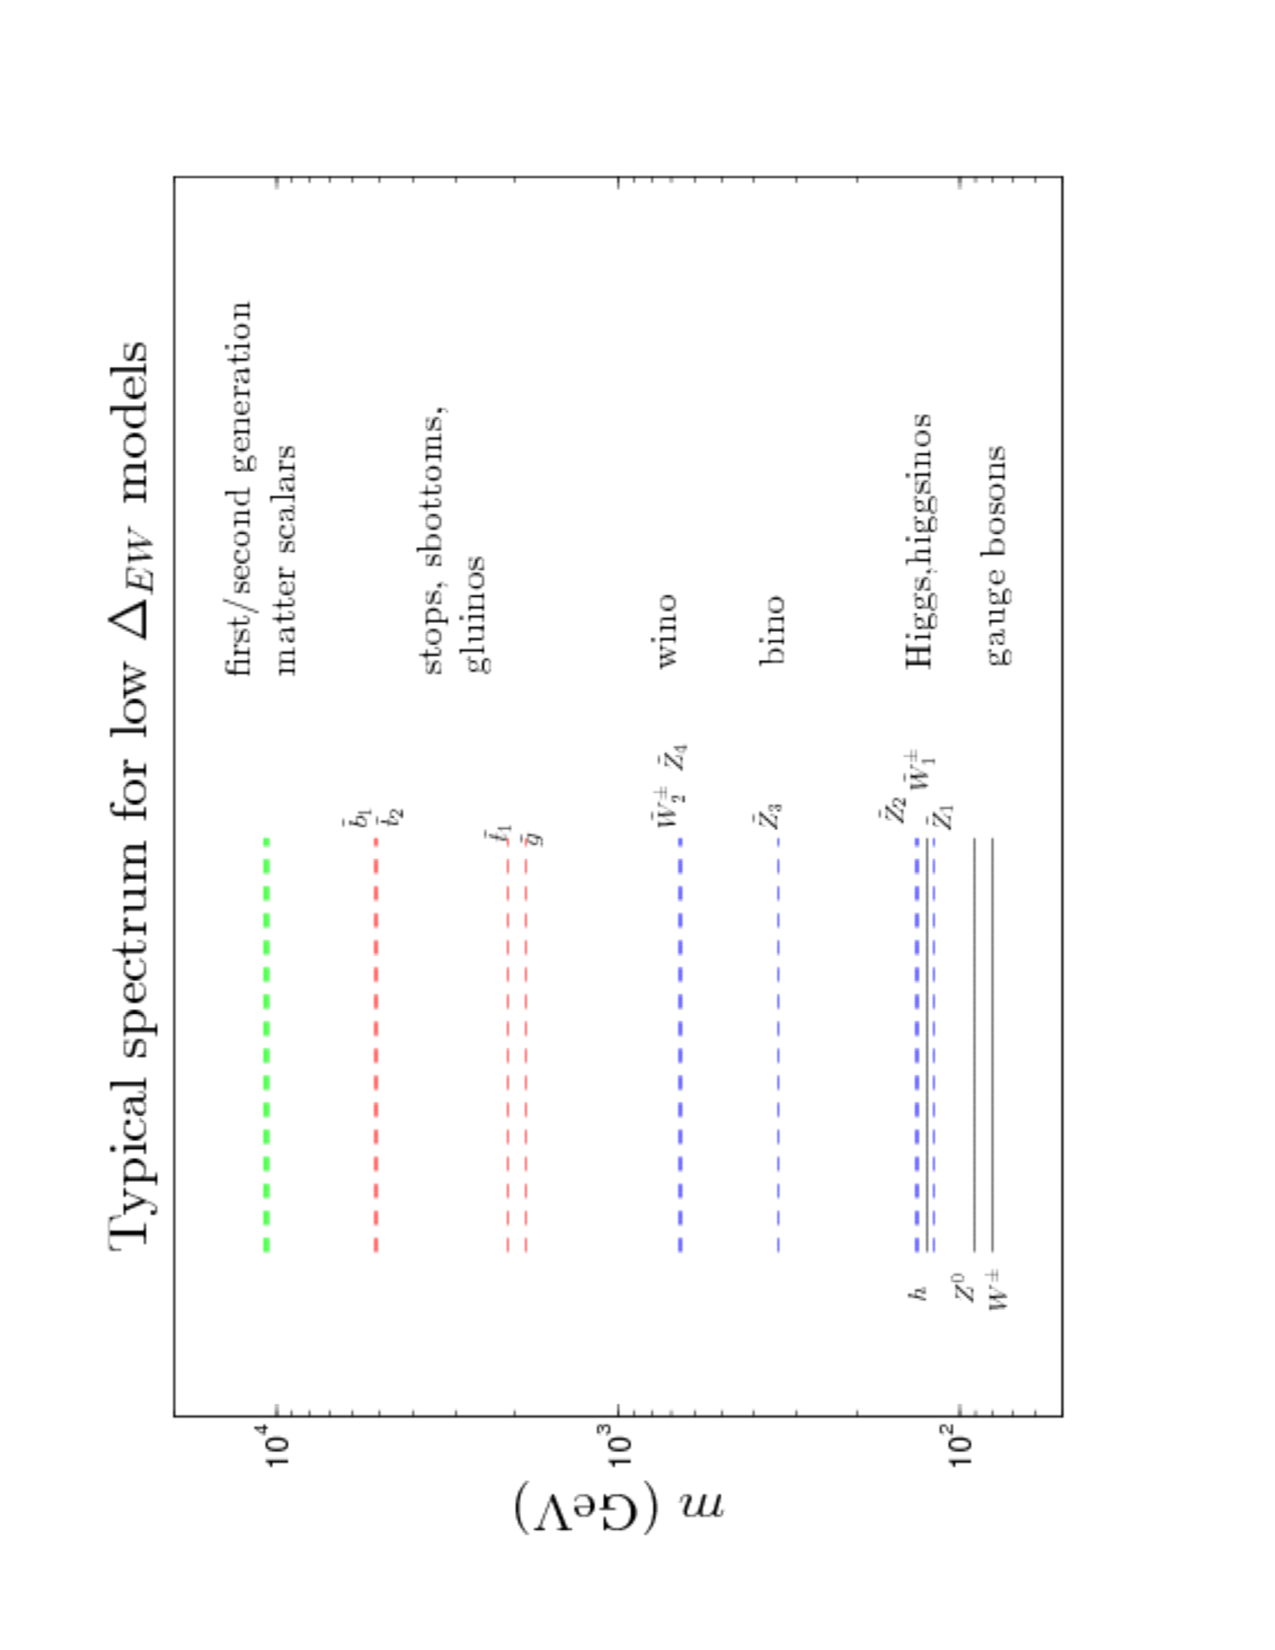
\includegraphics[scale=0.45,angle=270]{mass_hierarchy_xerxes_not.pdf}
        \caption{Typical sparticle mass spectra of RNS~\cite{Baer:2013gva}.}
        \label{fig:susy_RNS_mass_spectra}
    \end{center}
\end{figure}

%%%
%%%
%%%

\section{The non-universal Higgs mass model with two extra parameters}
\label{sec:susy_nuhm2}
The RNS can be generated from SUSY GUT type models using the non-universal Higgs masses model with two extra parameters (NUHM2)~\cite{Ellis:2002wv, Ellis:2002iu, Baer:2004fu, Baer:2005bu} leading to a low fine-tuning $\Delta_{EW}$ value at the electroweak scale and keeping electroweak naturalness.
The NUHM2 decouples the Higgs mass doublet parameters $m^{2}_{H_{u}}$ and $m^{2}_{H_{d}}$ at the GUT scale such that
%
\begin{equation}
    m^{2}_{H_{u}} \neq m^{2}_{H_{d}} \neq m^{2}_{0}(m_{\text{GUT}}) \quad ,
    \label{eq:susy_nuhm2_decouple}
\end{equation}
%
and usually uses the weak scale parameters $\mu$ and $m_{A}$ to replace the $m^{2}_{H_{u}}$ and $m^{2}_{H_{d}}$.
%
\begin{align}
    \mu^{2} &= \frac{m^{2}_{H_{d}} - m^{2}_{H_{u}}\tan^{2}\beta}{\tan^{2}\beta - 1} - \frac{m^{2}_{Z}}{2} \quad ,\\
    m^{2}_{A} &= m^{2}_{H_{d}} + m^{2}_{H_{u}} + 2\mu^{2} \quad ,
    \label{eq:susy_weak_scale_parameters}
\end{align}
%
If the value of NUHM2 free parameters are chosen as the following ranges
%
\begin{itemize}
    \item The matter scalar mass $m_{0} \sim 1$ to 7~{\TeV},
    \item The soft SUSY breaking gaugino mass $m_{1/2} \sim 0.3$ to 1.5~{\TeV},
    \item The trilinear SUSY breaking parameter $A_{0} \sim \pm(1$ to $2) m_{0}$,
    \item The  ratio of the Higgs field vacuum expectation value $\tan\beta \sim 5$ to 50,
    \item The superpotential Higgs mass $\mu \sim 100$ to 300~{\GeV},
    \item The pseudoscalar Higgs boson mass $m_{A}$ is varied,
\end{itemize}
%
then the low EWFT can be achieved while maintaining the SUSY spectrum in the range $123 < \mH < 127$~{\GeV}.
Compared with the well-known mSUGRA/CMSSM models which have the lowest $\Delta_{EW} \sim 200$, the $\Delta_{EW}$ in the NUHM2 model is only $\sim$10.
The NUHM2 is expected to form the the effective theory for energies lower than $m_{GUT}$ resulting from $SU(5)$ or general $SO(10)$ grand unified theories.
Detailed scans for the NUHM2 parameter space with low EWFT have been performed in~\cite{Baer:2013xua}.
The NUHM2 parameter values used in this analysis were set to $m_{0} = 5$~{\TeV}, $A_{0} = -1.6 m_{0}$, $\tan\beta = 15$, $m_{A} = 1$~{\TeV}, $\mu = 150$ such that sign($\mu$) $> 0$, and $m_{1/2}$ are varied from 350 to 800~{\GeV}.
These parameter choices lead to low EWFT (electroweak naturalness) and predict final state signatures that allow large background rejection while retaining high signal efficiency.
Although the kinematics of NUHM2 are very similar to the simplified Higgsino model in compressed scenarios, the primary differences between the two models exist in the mass spectra, cross-sections, and branching ratios.

\begin{figure}[htb]
    \begin{center}
        % 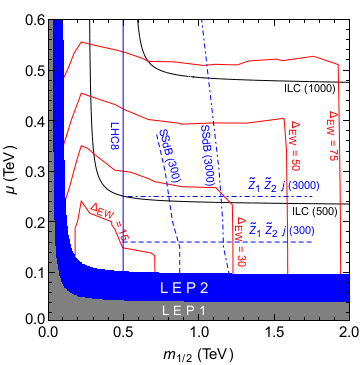
\includegraphics[scale=0.7]{mumhf.png}
        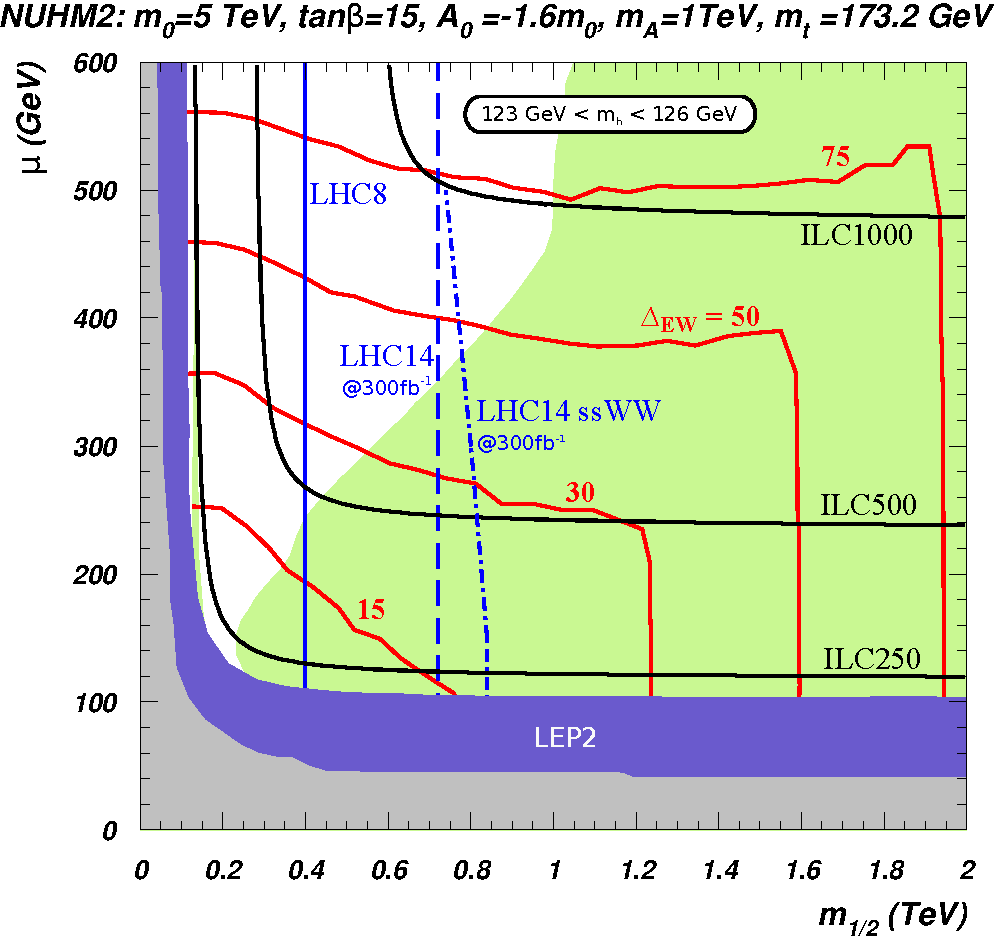
\includegraphics[scale=0.7]{nuhm2_muvmhf_tb10_n16_m05000_fi3.pdf}
        \caption{The $\Delta_{EW}$ contours in the $m_{1/2}$ vs $\mu$ plane of NUHM2 model for $m_{0} =  5$~{\GeV}, $\tan\beta = 15$, $A_{0} = -1.6 m_{0}$, and $m_{A} = 1$~{\TeV}~\cite{Baer:2016usl}.
        The gray and blue shaded regions are excluded by the LEP1 and LEP2 searches for chargino pair production.
        The region on the left hand side of the blue solid line is excluded by LHC $\sqrt{s} = 8$~{\TeV} gluino pair searches.}
        \label{fig:susy_mumhf}
    \end{center}
\end{figure}

Figure~\ref{fig:susy_mumhf} shows the $m_{1/2}$ vs $\mu$ plane of NUHM2 model for $m_{0} =  5$~{\GeV}, $\tan\beta = 15$, $A_{0} = -1.6 m_{0}$, and $m_{A} = 1$~{\TeV}.
The gray and blue regions are excluded by searches for chargino pair production at LEP1 and LEP2.
The area to the left of the blue solid line is excluded by the $\widetilde{g} \widetilde{g}$ production at the LHC with $\sqrt{s} = 8$~{\TeV}.
The contours for $\Delta_{EW} = 15, 30, 50, 70$ are shown.
The $\widetilde{\chi}^{0}_{2} \widetilde{\chi}^{0}_{1}$ with one ISR jet production where $\widetilde{\chi}^{0}_{2} \to \ell^{+} \ell^{-} \widetilde{\chi}^{0}_{1}$ is labeled by two horizontal dashed contours at 300 \ifb and 3000 \ifb, respectively\footnote{The $\widetilde{\chi}^{0}_{1}$ is indicated by $\widetilde{Z}_{1}$ and the $\widetilde{\chi}^{0}_{2}$ is indicated by $\widetilde{Z}_{2}$ in the plot.}.
The $\widetilde{\chi}^{0}_{2} \widetilde{\chi}^{0}_{1}$ with one ISR jet is accessible in nearly the entire $\Delta_{EW} < 30$ region.
For comparison, the reach of the International Linear Collider (ILC) with $\sqrt{s} = 0.5$ and 1~{\TeV} are shown.
Thus, the RNS, which accommodates the electroweak naturalness, can be either discovered or ruled out by the LHC plus ILC searches.
